114. Первые две прямые пересекаются в точке $(0;0).$ Найдём точку пересечения первой прямой и третьей: $\begin{cases}y=\cfrac{4}{3}x,\\ x+y=7.\end{cases}
\Leftrightarrow \begin{cases}y=\cfrac{2}{3}x,\\ x+\cfrac{4}{3}x=7.\end{cases}
\Leftrightarrow \begin{cases}y=4,\\ x=3.\end{cases}$ Найдём точку пересечения второй прямой и третьей: $\begin{cases}y=6x,\\ x+y=7.\end{cases}
\Leftrightarrow \begin{cases}y=6x,\\ x+6x=7.\end{cases}
\Leftrightarrow \begin{cases}y=6,\\ x=1.\end{cases}$ Таким образом, искомый треугольник имеет вершины в точках $(0;0),\ (3;4),\ (1;6).$\\
\begin{figure}[ht!]
\center{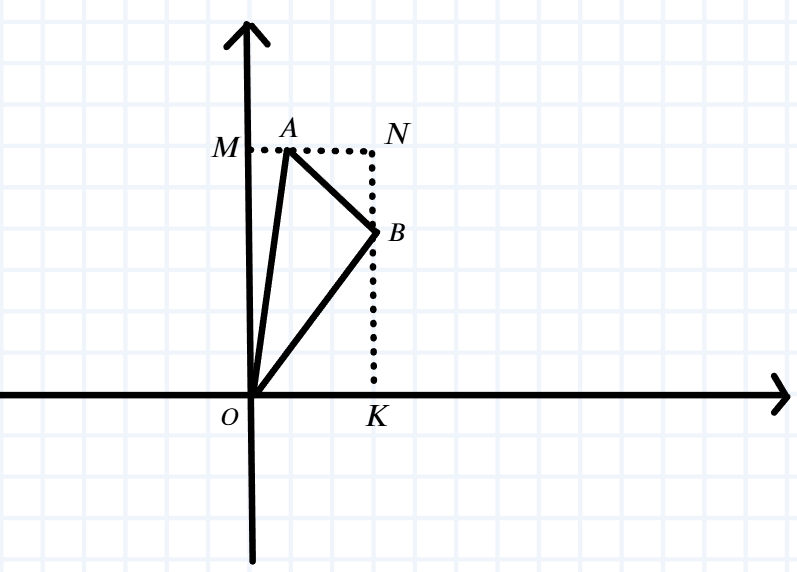
\includegraphics[scale=0.35]{g9-1001.png}}
\end{figure}\\
Достроив треугольник до прямоугольника, найдём его площадь: $S_{\Delta AOB}=S_{OMNK}-S_{\Delta OMA}-S_{\Delta ANB}-S_{\Delta OBK}=
3\cdot6-1\cdot6:2-2\cdot2:2-3\cdot4:2=7.$\\
